\chapter{Úvod}
%\addcontentsline{toc}{chapter}{Úvod}
\label{sec:uvod}

Strategické hry jsou žánrem, ve kterém hráči využívají svých mentálních schopností, především taktického a~strategického myšlení, pro porážku jednoho či více nepřátel. Ve většině případů se strategické hry zabývají tématem války. Takto popisuje strategické Ernest Adams ve své knize \textit{Fundamentals of Game Design} \citep[str.~419]{book:gamefund}

Žánr strategických her obsahuje mnoho poddruhů s~velice rozdílnými nároky jak na hráče, tak na vývojové prostředí a~na vývojáře samotného. Prvním kritériem pro rozdělení strategických her je, zda se hra odehrává jako posloupnost diskrétních tahů, nebo zda se hra odehrává v~přímé závislosti na ubíhajícím reálném čase. Druhým kritériem je relativní četnost a~důležitost strategických rozhodnutí vůči taktickým rozhodnutím. Tato dvě kritéria použil Mark H. Walker \citep{site:stratg05} pro jejich rozdělení na tyto poddruhy:
\begin{itemize}
	\item \emph{Real-time strategy} (RTS) - reálný čas, strategická rozhodnutí,
	\item \emph{Real-time tactics} (RTT) - reálný čas, taktická rozhodnutí,
	\item \emph{Turn-based strategy} (TBS) - diskrétní tahy, strategická rozhodnutí,
	\item \emph{Turn-based tactics} (TBT) - diskrétní tahy, taktická rozhodnutí.
\end{itemize}

Cílem této práce je vytvořit platformu umožňující tvorbu Real-time strategy (RTS)\footnote{Název "real-time strategy", poprvé použitý při propagaci hry Dune~II \citep{site:dune2}, je připisován prezidentu a~spoluzakladateli Westwood Studios \citep{site:westwood}, \emph{Brettu Sperrymu}. Toto studio následně využilo zkušenosti získané při tvorbě Dune~II pro vývoj jedné z~nejznámějších sérií RTS her, Command~\&~Conquer \citep{site:cmdcnq}.} her. V~následujících částech popíšeme rozdíly mezi poddruhy strategických her a~vymezíme podmnožinu, jejíž vývoj bude naše platforma podporovat. 

\subsubsection{Real-time strategy}
 RTS, v~překladu strategické hry probíhající v~reálném čase, jsou poddruhem strategických her ve kterém se změny stavu odehrávají v~přímé závislosti na změně času v~reálném světě. Reakce v~reálném čase jsou náročnější jak pro hráče, který je často nucen použít suboptimální strategii, tak pro hru samotnou, která musí provádět výpočet dalšího stavu v~omezeném čase. Stejně tak umělá inteligence, jakožto součást hry, musí reagovat na aktivity zbylých hráčů s~omezeným časem, což limituje množství dat a~složitost výpočtu, které může umělá inteligence použít. Z~tohoto důvodu je vývoj RTS her složitým procesem, spojujícím mnoho oborů, který se pokusíme zjednodušit vytvořením naší platformy.

Zbylé poddruhy strategických her neplánujeme v~naší platformě explicitně podporovat, ale nijak nevylučujeme, že bude možné do jisté míry využít naší platformu i~pro tvorbu těchto poddruhů strategických her. Zároveň je pro tvorbu RTS her výhodné znát příbuzné žánry, z~kterých je možno se inspirovat a~přebírat některé z~jejich mechanik. Z~tohoto důvodu ve zkratce popíšeme i~zbylé poddruhy.

\subsubsection{Real-time tactics}
Prvním příbuzným žánrem jsou \emph{Real-time tactics} (RTT) hry, někdy také nazývány fixed-unit real-time hry \citep{site:stratg02}, neboli hry s~pevným počtem jednotek probíhající v~reálném čase. Hlavním rozdílem, odlišující RTT od RTS, je omezení  strategických rozhodnutí a~větším důrazem na taktická rozhodnutí a~micromanagement jednotlivých jednotek. RTT hry nedovolují hráči tvorbu nových jednotek, stavbu budov či produkci surovin, hráč je tedy nucen s~jednotkami, které má na začátku souboje, vyhrát celý souboj.  Jedním z~příkladů čistě RTT her je série Blitzkrieg \citep{site:blitzkrieg}. Hráč začíná každou misi s~jednotkami, které si vybral před misí. Tyto jednotky jsou jediné, které bude moci v~průběhu mise využít, což nutí hráče použít svých taktických schopností a~maximalizovat účinnost těchto jednotek. 

\subsubsection{Turn-based strategy}
\emph{Turn-based strategy} jsou strategické hry, ve kterých změny stavu probíhají v~diskrétních tazích. Doba mezi tahy často není nijak omezena, což hráči umožňuje vymyslet optimální strategii. Oproti RTS tyto hry často omezují taktickou část problémů a~umožňují hráči soustředit se výhradně na strategickou část hry, tedy plánování budov, produkci surovin, vývoj technologií a~celkovou strategii pro jeho ekonomiku a~armádu. Příkladem tohoto žánru je série her Civilisation \citep{site:civ5}. Naše platforma nebude explicitně podporovat tahy, myslíme si však, že bude možné toto rozdělení do tahů vytvořit použitím platformou poskytovaných prostředků.

\subsubsection{Turn-based tactics}
Turn-based tactics umožňují hráči přímé ovládání několika málo jednotek, které v~každém tahu mohou provést jeden či více úkonů. Těmito úkony mohou být střelba na nepřátelskou jednotku, vyléčení přátelské jednotky, pohyb po mapě či například zničení terénu. Ukázkovým příkladem je série her X-COM \citep{site:XCOM}. Ve hře X-COM~2 hráč vlastní až malé desítky jednotek, z~kterých vybírá malou skupinu a~vysílá ji na jednotlivé mise. Při misi má každá jednotka v~každém tahu možnost vykonat dvě akce. Akce může být přesun o~omezenou vzdálenost, použití schopnosti či útok na nepřítele. Pro normální jednotky útok ukončuje tah dané jednotky a~hráč může provést tah následující. 

\subsubsection{Shrnutí}

Jak můžeme vidět, žánr strategických her zahrnuje hry s~velmi rozmanitými vlastnostmi a~požadavky. Z~tohoto důvodu se naše práce zaměří na podporu vývoje her jednoho konkrétního poddruhu, a~to RTS. Přestože naše platforma bude cílena na tvorbu tohoto poddruhu, nevylučujeme, že bude možné využít ji i~pro tvorbu her spadajících do jednoho ze zbylých poddruhů strategických her.


\section{RTS hry blíže}
Jak bylo řečeno výše, naše platforma bude navržena pro podporu vývoje RTS her. RTS hry jsou ovšem stále příliš velká množina s~příliš rozmanitými mechanikami na to, aby jedna platforma dokázala podporovat všechny možné RTS hry. Proto zde dále omezíme námi podporovanou podmnožinu RTS her.

Již od svého vzniku na konci osmdesátých let a~začátku devadesátých let minulého století obsahovaly RTS hry několik konceptů, které lze nalézt v~drtivé většině her tohoto žánru i~dnes. 

\noindent{Těmito koncepty jsou:}
%tady pouzivam stredniky pro oddeleni, protoze uvnitr jsou pouzity carky
\begin{itemize}
	\item výroba a~ovládání jednotek s~cílem ovládnutí části mapy a~zničení nepřátelských jednotek a~budov;
	\item stavba budov pro umožnění stavby nových druhů budov, jednotek či získání surovin;
	\item získávání surovin pro stavbu jednotek a~budov;
	\item výzkum nových technologií.
\end{itemize}

Tyto koncepty, jako základní kámen RTS her, se bude naše platforma snažit podporovat a~zjednodušit tvůrcům her jejich implementaci.

Hlavní inspirací pro tvorbu platformy, a~tím i~pro typ her, které bude platforma nejjednodušeji podporovat, byla hra Stronghold Crusader. Na této a~dalších hrách ukážeme v~následujících částech blíže základní principy RTS her a~námi podporované implementace těchto principů.

\done
\todo[Možná vynechat]{Možná vynechat}
\subsubsection*{Strategie vs. taktika}
Jedním z~hlavních problémů RTS her je pečlivé vyvážení kombinace strategie/macromanagementu a~taktiky/micromanagementu. Tyto pojmy bývají často špatně chápány a~někdy zaměňovány, pokusíme se je proto konkrétně definovat. Strategií míníme rozhodnutí týkající se globálního průběhu hry. Taktika naopak zahrnuje konkrétní pozice konkrétních jednotek, jejich pohyb po mapě a~spolupráci v~jedné bitvě. 

Mezi strategická rozhodnutí v~RTS hrách patří kupříkladu které budovy hráč postaví, v~jakém pořadí dané budovy postaví, které suroviny bude produkovat, které suroviny vynechá, které jednotky bude rekrutovat a~které vynechá. Tato 3 rozhodnutí jsou úzce propojena, protože výběr surovin určuje budovy, které bude hráč schopen postavit a~typy jednotek, které bude moci zrekrutovat. Stejně tak výběr budov určuje suroviny, které hráč může produkovat a~typy jednotek, které může zrekrutovat. 

Taktika/micromanagement je v~RTS hrách reprezentován ovládáním jednotek, jejich přesné pozice, pohybu, směru útoku, používání schopností atd. Micromanagement lze ale vidět i~v~ekonomické stránce hry, kdy hráč 

Nejlepším příkladem pro rozlišení pojmu strategie a~taktiky je série her Total War \citep{site:totalwar}, které kombinuje mód tahové strategie s~módem real-time tactics (RTT). V~jedné části hry hráč přebírá kontrolu nad celým svým národem, rozhoduje, které budovy budou ve kterých městech postaveny, které jednotky budou rekrutovány a~kde budou které armády umístěny. V~druhé části, při souboji nepřátelských armád, hráč přebírá kontrolu nad konkrétní armádou a~ovládá jednotlivé bataliony, jejich umístění, pohyb a~útoky v~reálném čase.

Naše platforma nemá za cíl nijak omezovat možnosti vytvářených her v~rámci jejich zaměření na taktiku či strategii. Toto rozhodnutí chceme nechat čistě na uživateli naší platformy.

\subsection{Mapy}
\label{sec:mapy}
Reprezentace herní mapy je jedním z~hlavních rozhodnutí při tvorbě RTS her. Hlavní funkcí herní mapy je reprezentovat terén pro pohyb jednotek a~stavbu budov. 
Tato funkce může zahrnovat neprostupné části mapy, několik různých druhů terénu prostupné různým druhům jednotek či části mapy ovlivňující rychlost pohybu jednotek.
Při stavbě budov je pak často omezen typ terénu, na kterém je hráč schopen danou budovu postavit. 
Vzhledem k~uzavřenosti většiny RTS her je složité zjistit, jak je v~každé z~nich herní svět reprezentován, z~pozorovatelného vnějšího chování lze ale odvodit několik základních druhů reprezentací. 

Nejstarší a~nejjednodušší reprezentací je rozdělení mapy na stejně velké dlaždice. Tyto dlaždice mohou být různých tvarů, nejčastěji jsou však čtvercové či hexagonální. Příkladem takovéto reprezentace je právě hra Stronghold Crusader \citep{site:strongholdcrus}, podle které chceme naši platformu modelovat. Jak je vidět na obrázku  \ref{fig:tiletype}, herní mapa je viditelně rozdělena na stejně velké čtvercové dlaždice. Dále můžeme vidět, že je kamera orientována diagonálně vůči dlaždicím. Účelem této orientace je skrytí toho, že je mapa složena z~dlaždic. Každá dlaždice je nějakého typu, který určuje její vzhled, což můžeme vidět v~části zvýrazněné červenou barvou. Vidíme zde řady pěti dlaždic stejného typu, oddělené vždy jednou dlaždicí pouštního typu. Můžeme si všimnout, že i~dlaždice stejného typu mohou mít několik různých vzhledů. Typ dlaždice je dále využíván jako omezení při stavbě budov, kde například kamenolom lze postavit pouze na dostatečném počtu dlaždic typu kámen. Toto můžeme vidět v~části označené modrou barvou, kde se hráč pokouší umístit budovu, která ovšem nemůže být postavena na dlaždicích typu mokřadu. Dlaždice tohoto typu jsou proto zvýrazněny červenou barvou v~rámci půdorysu budovy. Dále můžeme v~horní části ukázky vidět dlaždice s~rozdílnou výškou od okolního terénu, tvořící nedostupnou oblast mapy. Dále můžeme vidět pro jednotky neprostupný typ dlaždic obsahujících vodu. Uprostřed obrázku poté vidíme velkou oblast kamení a~železa, kde oblast kamení ukazuje texturu kvalitně skrývající složení mapy z~dlaždic, naopak na oblasti železa jasně vidíme hranice jednotlivých dlaždic, především ve směru z~levého dolního rohu do pravého horního rohu.

\begin{figure}[h]
	\centering
	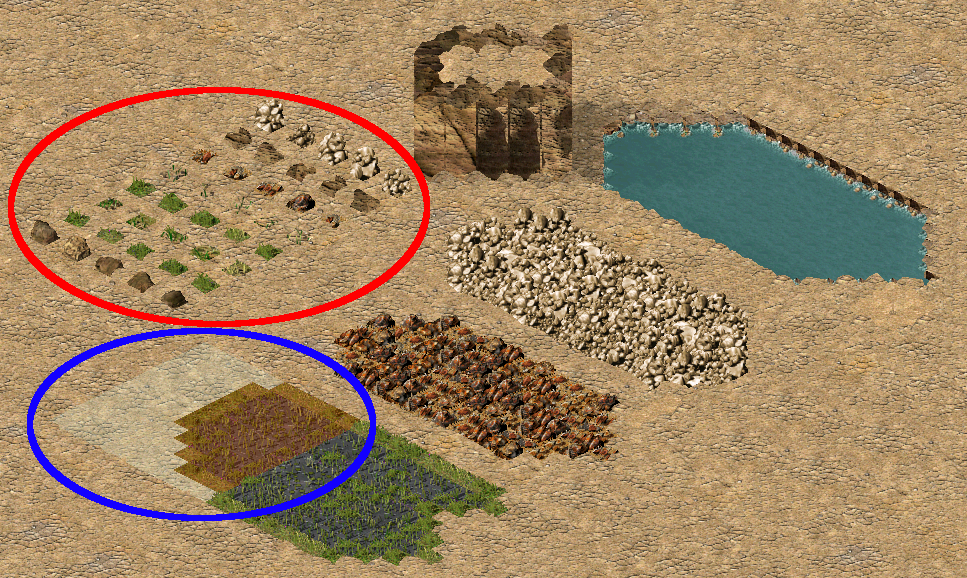
\includegraphics{strongholdtiles}
	\caption{Ukázka dlaždic ve hře Stronghold Crusader}
	\label{fig:tiletype}
\end{figure}

Na každé dlaždici může být postavena až na výjimky nejvýše jedna budova a~stát nejvýše jedna jednotka. Při pohybu jednotek není tato vlastnost dodržována, lze tedy jednotky přesouvat přes dlaždice na kterých již jiná jednotka stojí. 

Naše platforma bude podporovat rozšířenější verzi tohoto druhu mapy, ve které nebudeme vynucovat limity na počty jednotek a~budov na jedné dlaždici. Tato omezení budou přenechána pro implementaci tvůrcem her využívajících naší platformu a~bude vytvořeno rozhraní pro co nejjednodušší implementaci těchto limitů. 

\noindent{Naše platforma bude podporovat mapu s~těmito vlastnostmi:}
\begin{itemize}
	\item[\textbf{M1:}] terén rozdělený na čtvercové dlaždice,
	\item[\textbf{M2:}] dlaždice s~různou výškou,
	\item[\textbf{M3:}] dlaždice různých typů,
	\item[\textbf{M4:}] možnost dotazovat se na jednotky nacházející se na dlaždici,
	\item[\textbf{M5:}] možnost dotazovat se na budovy postavené na dlaždici.
\end{itemize}
\subsection{Jednotky}
\label{sec:jednotky}
Jednotky jsou základním nástrojem hráče pro boj s~nepřítelem. Pohybem po mapě, poškozováním ostatních jednotek a~ničením budov jednotky umožňují hráči vést souboj s~protivníkem, získat strategickou výhodu a~následně vyhrát hru. 

\subsubsection{Pohyb}
Hlavním odlišujícím prvkem jednotek od budov je jejich schopnost pohybu. Pohyb jednotky je určen jejím typem, kde každý typ jednotek může procházet jinými typy terénu, pohybovat se nad terénem, na vodě či pod vodou. Naše platforma bude podporovat pohyb jednotek kdekoli nad terénem, navíc bude tvůrcům poskytnuta komponenta umožňující chůzi po terénu, neboť je to nejčastější způsob pohybu. 

Pohyb jednotek je nejčastěji řízen hráčem, ať už na úrovni příkazů jednotlivým jednotkám, tak na úrovni slučování jednotek do skupin a~ovládání těchto skupin. Naše platforma bude umožňovat jak ovládání jednotlivých jednotek, tak celých skupin. Dále umožníme vývojáři přidat složitější ovládání, například slučování do permanentních formací a~následné ovládání těchto formací. 

V některých hrách existují také jednotky, které se mohou své schopnosti pohybu vzdát a~stát se budovu, buď dočasně, nebo trvale. Příkladem takovéto jednotky/budovy mohou být budovy Nočních elfů ze hry Warcraft 3 \citep{site:warcraft3}. Tyto entity jsou stavěny jako budovy, tedy jsou umístěny do světa a~postaveny jednotkou, stejně jako u~všech ostatních ras. Následně je ale hráči umožněno, pomocí speciální ability těchto budov, změnit je dočasně na jednotky a~pohybovat s~nimi či je dokonce použít pro boj. V~tomto módu ale ztrácí všechny funkce budov, tedy není možné je použít pro sběr surovin či produkci jednotek. Následně je možné znovu je zakořenit, čímž získávají zpět své funkce budovy.  Naše platforma by měla takovéto jednotky/budovy také podporovat. 

\subsubsection{Umělá inteligence}

Ve velké části RTS her jsou jednotky schopny do určité míry autonomního rozhodování bez zásahu hráče, od střelby na cíl, který se ocitne v~jejich dostřelu, po vyhledání krytu, pokud jsou pod palbou. 

Jako příklad jednoduché umělé inteligence jednotek můžeme vzít hry Starcraft \citep{site:starcraft} a~Warcraft \citep{site:warcraft3} od společnosti Blizzard \citep{site:blizz}. Zde se jednotky chovají velice předvídatelně, splňují přesně hráčovi rozkazy a~nedělají nic navíc, což James Lantz \citep{site:gamasutra01} označuje jako jeden z faktorů, které umožnili hře Starcraft II vytvořit jednu z~prvních masivních e-sport scén na světě.



Dobrým příkladem jednotek s~vysokou autonomií je série Company of Heroes \citep{site:COH}, kde jednotky automaticky vyhledávají krytí, rozutečou se, pokud jsou pod palbou dělostřelectva, a~v~případě příliš velkých ztrát utečou z~boje. Příklad tohoto chování můžeme vidět na obrázku \ref{fig:cohai}. V~levé části vidíme skupinu jednotek, útočících na nepřátelskou jednotku mimo obraz ve směru červené šipky. Na prostřední části můžeme vidět, že po zničení nepřátel se jednotka začala přesouvat ve směru modré šipky, nejspíše pro získání lepšího krytí a~lepší palebné pozice vůči zbývajícím nepřátelským jednotkám. Tento přesun je vykonán bez zásahu hráče, jak můžeme vidět díky modré ikoně nad jednotkou, která značí, že jednotka není zvolena hráčem a~není jím tedy ovládána. Oproti tomu v~pravé části můžeme vidět, že jednotka hráčem označena je díky bílé barvě ikony nad jednotkou. Vidíme, že hráč vydal rozkaz pro přesun zpět, zvýrazněný zeleně. Tato reakce byla vynucena umělou inteligencí jednotky, která se sama od sebe rozeběhla ve směru nepřátelských linií a~donutila hráče reagovat. Jak vidíme, autonomie má svou cenu, a~to v~nepředvídatelnosti chování jednotek. Při jednoduché umělé inteligenci jednotek je hráč schopen předvídat jejich chování a~využít ho pro svůj prospěch. Naopak při složité umělé inteligenci, jako právě v~případě Company of Heroes, je hráč často nucen provést více pokusů při vydávání rozkazu, či vydávat rozkazy pro negaci automatického chování jednotky, protože není schopen toto chování jednoduše odhadnout. Tato skutečnost činí hry často realističtější, protože simuluje chování reálných vojáků, kteří rozkaz interpretují a~implementují podle svého, není ale vhodná pro souboje více hráčů, a~už vůbec né více hráčů na profesionální úrovni.

\begin{figure}[h]	
	\centering
	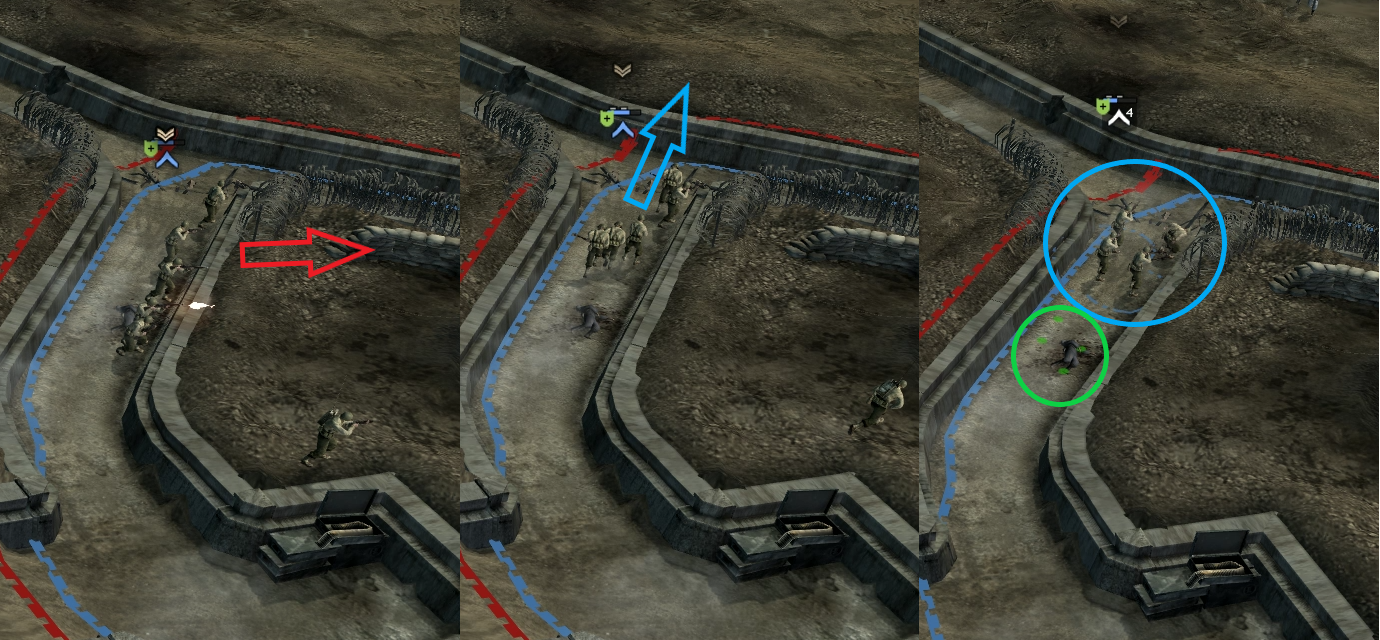
\includegraphics[scale=0.35]{cohai}
	\caption{Ukázka autonomního chování jednotek ve hře Company of Heroes \citep{site:COH}}
	\label{fig:cohai}
\end{figure}

Platforma bude umožňovat vykonat libovolný kód v~rámci každého výpočtu stavu každé jednotky, bude tedy pouze na vývojáři, zda se budou jednotky chovat jednoduše a~předvídatelně, nebo zda budou vykonávat složité, avšak nepředvídatelné úkony bez hráčova vědomí. Pro ulehčení vývoje bude platforma poskytovat předpřipravené komponenty, umožňující základní úkony jako střelbu na cíl, pohyb po mapě a~útok na blízko.

\subsubsection{Produkce}

Jednou z~vlastností definujících RTS hry je možnost produkce nových jednotek. Existuje několik systémů produkce jednotek, úzce svázaných se systémem surovin v~dané hře. (viz. \ref{sec:suroviny})  Od kontinuální produkce, kde hráč zvolí produkované jednotky a~suroviny jsou spotřebovávány v~průběhu produkce, po diskrétní produkci, kde hráč musí vlastnit všechny suroviny potřebné pro výrobu dané jednotky při začátku produkce a~všechny suroviny jsou odečteny v~jeden okamžik. Kontinuální systém umožňuje hráči naplánovat produkci armády v~předstihu, i~když v~daném okamžiku nevlastní dostatečné suroviny. Naopak při diskrétní produkci je hráč nucen čekat do chvíle, kdy má všechny suroviny, a~až poté může začít s~produkcí. Naše platforma se pokusí podporovat oba systémy. Bude záležet pouze na tvůrci hry, jak se k~surovinám a~produkci jednotek zachová a~který z~těchto systémů bude implementovat.

Počet jednotek je často limitován, jak pro účely vyvážení hry, tak pro omezení zátěže hardwaru. Z~hlediska vyvážení síly jednotek umožňuje limit na počet jednotek předejít tzv. \uv{Zergu}, kdy hráč vytvoří obrovské množství levných jednotek, které následně převálcují jakýkoli odpor. Z~hlediska hardwarové náročnosti je účel limitu vcelku zřejmý, protože každá jednotka zabírá určité množství paměti a~výpočetního výkonu. Stronghold Crusader omezuje počet jednotek na 1000 pro každého hráče. Toto omezení se jeví především jako limit na hardwarovou náročnost hry. Naše platforma žádné explicitní limity nestanovuje, avšak v~uživatelské dokumentaci pro vývojáře budeme silně doporučovat stanovení limitů na počet budov, jednotek a~projektilů. Za tímto účelem umožníme vývojáři při vytvoření každé jednotky, budovy či projektilu učinit rozhodnutí, zda je vytvoření možné a~případně toto vytváření zrušit. 

Hráč často začíná s~malým počtem jednotek, jejichž účelem je zamezit tzv. \uv{Rush} strategii, ve které je cílem vytvořit co nejrychleji co možná nejvíce levných jednotek a~zničit nepřítele ještě před tím, než je schopen začít produkovat své jednotky. Ve hře Stronghold Crusader hráč začíná každou hru s~několika lučišníky a~kopiníky, jejichž počet je určen v~nastavení před začátkem hry. Toto bude v~naší platformě umožněno přidáváním jednotek v~rámci editace mapy, případně bude tvůrce hry schopen umožnit hráči určit počty jednotek před začátkem hry pomocí grafických elementů v~uživatelském rozhraní a~následně při začátku hry vytvořit požadované množství jednotek. Tyto jednotky bude poté hráč vlastnit již na počátku hry.

\subsubsection{Boj}

V drtivé většině RTS her mají jednotky tzv. \uv{hit pointy} , zkráceně \textit{HP}, které určují počet zásahů, které může jednotka obdržet než bude zabita. S~každým zásahem jsou poté tyto \textit{HP} odečítány a~v~okamžiku, kdy je jednotka poškozena na 0 \textit{HP} je zabita. Naše platforma bude tento systém samozřejmě podporovat, ale nebude ho nijak explicitně vyžadovat, bude tedy tvůrci umožněno použít jakýkoli jím implementovaný systém. 

Jednotky mohou obdržet poškození z~mnoha zdrojů, nejčastěji však útokem z~blízka (tzv. \textit{meele}) či z~dálky (tzv. \textit{ranged}). Útok na blízko je omezen dosahem, rychlostí útoků a~velikostí uděleného poškození. Naše platforma bude podporovat komponentu poskytující útoky na blízko právě s~těmito parametry. Útok na dálku lze rozdělit do dvou typů, tzv. \textit{hit-scan} a~\textit{projektily}. První typ je reprezentován například laserovými zbraněmi, které v~okamžiku výstřelu urazí celou vzdálenost, dokud nenarazí na terén či nějakou entitu (budovu či jednotku). Druhý typ v~okamžiku výstřelu vytvoří projektil, který se v~průběhu času pohybuje herním světem, dokud také nenarazí na terén či nějakou entitu. Naše platforma bude podle předlohy Strongholdu Crusader podporovat především projektilové útoky. Za tímto účelem bude vytvořena komponenta umožňující střelbu projektilů, dále projektily samotné, simulace jejich letu a~především možnost výpočtu pro střelbu na pohyblivý cíl. Hit-scan útoky nebudou přímo podporovány, mělo by však být umožněno tvůrci hry tento typ útoků implementovat manuálně.

\subsubsection{Shrnutí požadavků}
\noindent{Naše platforma bude podporovat jednotky s~těmito vlastnostmi:}
\begin{itemize}
	\item[\textbf{J1:}] pohyb jednotek volně kdekoliv nad terénem,
	\item[\textbf{J2:}] podpora pohybu po terénu,
	\item[\textbf{J3:}] ovládání jednotek a~skupin jednotek,
	\item[\textbf{J4:}] rozšiřitelnost o~složitější ovládání,
	\item[\textbf{J5:}] podpora jednoduché i~složité umělé inteligence v~podobě vykonání libovolného kódu,
	\item[\textbf{J6:}] podpora diskrétní i~kontinuální produkce jednotek,
	\item[\textbf{J7:}] přidávání jednotek při editaci mapy,
	\item[\textbf{J8:}] přidávání jednotek při startu hry,
	\item[\textbf{J9:}] podpora systému hit-pointů,
	\item[\textbf{J10:}] útoky na blízko i~na dálku,
	\item[\textbf{J11:}] simulace projektilů.
\end{itemize}

\done
\todo[Přeuspořádat]{Lépe uspořádat sekci o~budovách}
\subsection{Budovy}
\label{sec:budovy}
Stavba budov představuje jednu z~hlavních prezentací hráčovi strategie. Podle postavených budov lze často vcelku přesně odhadnout, jakou strategii hráč zvolil, čímž je umožněno nepřátelům reagovat a~adaptovat svou strategii odpovídajícím způsobem. 
Při volbě strategie lze ale narazit na problém, kdy je hráč nucen zvolit svou strategii před tím, než nalezne protivníky a~tedy před tím, než může vidět jejich strategii. Tento problém je velmi výrazný při tzv.  \uv{rock-paper-scisors}  strategiích, popisovaných například v knize Fundamentals of Game Design \citep[str.~329]{book:gamefund}. Hlavní myšlenkou tohoto návrhu her je situace, kdy strategie 1 poráží strategii 2, strategie 2 poráží strategii 3 a~strategie 3 poráží strategii 1. Ve chvíli kdy naše hra umožňuje hráči zvolit pouze jednu z těchto strategií bez viditelnosti protivníkovy strategie, degeneruje hra v~loterii, zda hráč náhodně vybere správnou strategii porážející tu vybranou nepřítelem. Jedním z~řešení tohoto problému, navrhovaných v článku od studia Oxeye \citep{site:oxeye03}, je co nejmenší rozdíl v~síle prvních úrovní technologie, což umožní hráčům reagovat a~změnit svoji strategii před tím, než je rozdíl mezi jejich silami neúnosně velký. Dalším možným řešením, použitým ve Stronghold Crusader \citep{site:strongholdcrus}, je neskrývat před hráčem nepřítelovu strategii. Toto řešení lze použít v~různé míře, od odhalení nepřátelských budov po úplné odkrytí celé mapy, tedy pozice všech jednotek i~budov, ať už přátelských, nepřátelských či neutrálních. Naše platforma použije toto poslední řešení, kdy budeme hráč vidět všechny jednotky a~budovy všech hráčů.

\noindent{Budovy mají ve hrách mnoho funkcí, mezi které patří například:}
\begin{itemize}
	\item Produkce jednotek
	\item Vylepšování jednotek
	\item Produkce surovin
	\item Uskladnění surovin
	\item Obrana
	\item Stavba budov
	\item Zkoumání technologií
\end{itemize}


Naše platforma se pokusí co nejvíce zjednodušit implementaci těchto funkcí poskytnutím programátorského rozhraní pro umístění budov a~jednotek do herního světa, přidání a~odebrání surovin hráči či střelbu projektilů. Dále umožníme tvůrci her přístup ke grafickému rozhraní, do kterého bude možné umístit okna, tlačítka a~další elementy, které následně použitím programátorské rozhraní budou schopné implementovat všechny zmíněné funkce budov.  

Jak již bylo řečeno v~sekci o~jednotkách \ref{sec:jednotky}, naše platforma bude nechávat volbu mezi kontinuální a~diskrétní produkcí jednotek na tvůrci hry. Budeme se tedy snažit do co největší míry podporovat oba tyto způsoby. 

\subsubsection{Obrana}

Obrana bude podporována v~podobě komponent, které umožní budovám jak útok na blízko, jako v~případě pastí ve hře Stronghold Crusader \citep{site:strongholdcrus}, tak na dálku, jako například obranné věže ve hře Warcraft~3 \citep{site:warcraft3}. 

Dále v~rámci funkce obrany umožňují v~některých hrách budovy jednotkám pohybovat se po nich. Jak můžeme vidět na obrázku \ref{fig:unitsonbuildings} ze hry Stronghold Crusader \citep{site:strongholdcrus}, jednotky mohou být umístěny na hradbách, věžích, bránách či na tvrzi. Na obrázku můžeme vidět různé typy jednotek, umístěné po obvodu hradu pro jeho obranu. Jak bylo řečeno v~části o~jednotkách, naše platforma bude umožňovat neomezený pohyb jednotkami, tedy i~ve vzduchu, na budovách či skrz budovy. Protože se pohyb po budovách vyskytuje ve velkém množství RTS her, poskytne platforma možnost rozšíření terénu o~plochu budov a~komponentu umožňující chůzi po těchto plochách.

Umístění na budovách poskytuje jednotkám ochranu před nepřátelskými jednotkami útočícími na blízko, které se musí nejdříve dostat do blízkosti cíle, než zaútočí. 

\begin{figure}[h]	
	\centering
	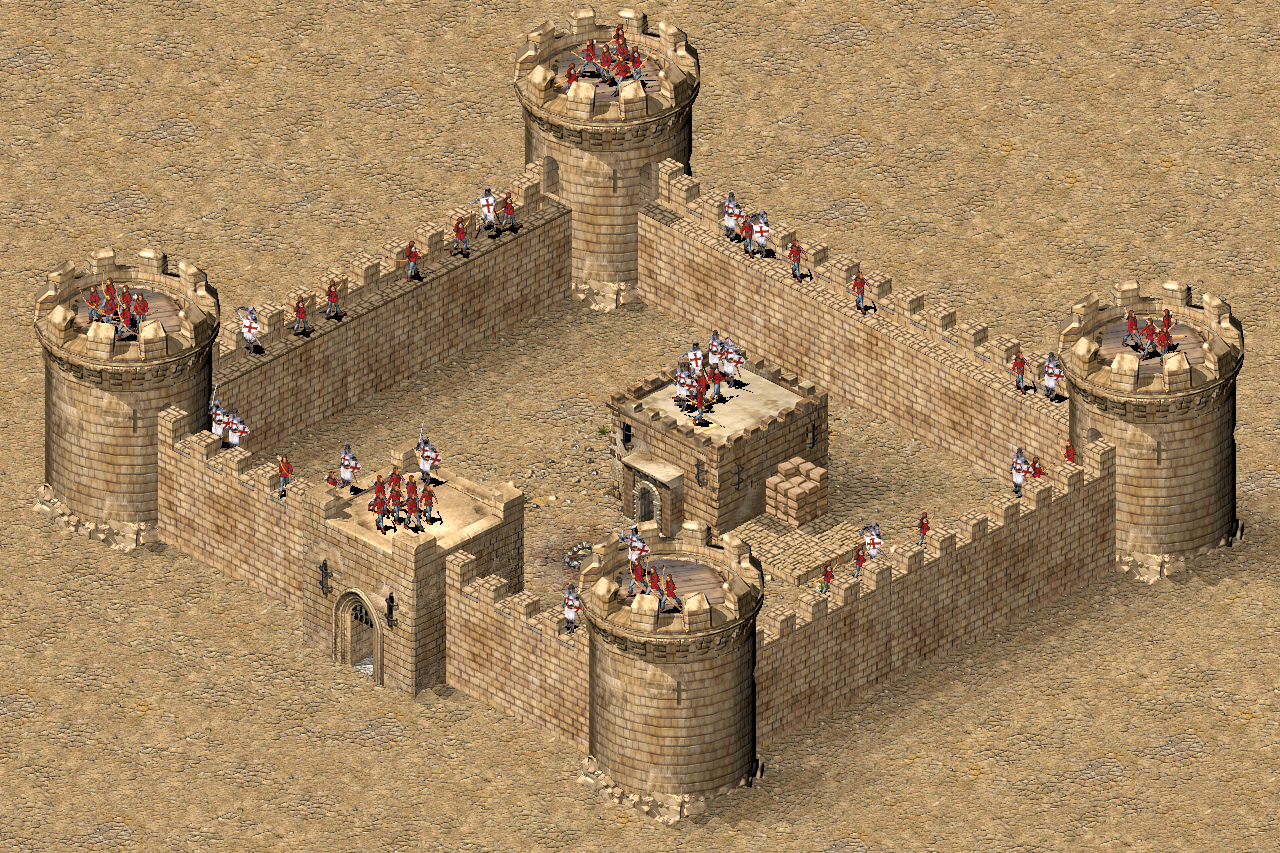
\includegraphics{unitsonbuildings}
	\caption{Jednotky umístěné na budovách ve hře Stronghold Crusader \citep{site:strongholdcrus}}
	\label{fig:unitsonbuildings}
\end{figure}

V některých hrách, kde bohužel Stronghold Crusader \citep{site:strongholdcrus} není jednou z~nich, poskytuje vyvýšení nad terén jednotkám větší dostřel. Tento efekt nemusí být omezen pouze na vyvýšení pomocí budov, ale lze ho dosáhnout už při rozdílných výškách terénu, na kterém je umístěn střelec a~jeho cíl, obecněji na rozdílu výšky pozice střelce a~cíle, pokud se střelec nemusí pohybovat přímo po terénu. Naše platforma bude podporovat realistické chování projektilů splňující tuto vlastnost. 

\done
\todo{zničitelnost}
\done
\todo{různé druhy poškození}

Budovy, podobně jako jednotky, mají ve většině her určitý počet tzv. \uv{hit pointů} , které určují počet zásahů, které může budova obdržet před tím, než bude zničena. Navíc oproti jednotkám mohou budovy často obdržet poškození pouze od omezené podmnožiny jednotek, nejčastěji pouze obléhacích strojů. Stejně jako u~jednotek přenecháme systém poškození na tvůrci hry. Naše platforma pouze umožní budově reagovat na zásah projektilem či zbraní, ať už snížením svých \textit{HP}, nebo ignorováním daného útoku v~případě že přišel od jednotky či projektilu, který danou budovu nemůže poškodit.


\subsubsection{Stavba budov}
\done
\todo{restrikce na umístění}
Budovy mají často restrikce, které je hráč nucen splnit před stavbou budovy. Tyto restrikce mohou sahat od reliéfu a~typu terénu, přes existenci jiných budov ve stejném místě, po vlastnictví určitého množství surovin či typu jednotek. Naše platforma umožní tvůrci před stavbou budovy zjistit stav všech těchto typů restrikcí a~případně vetovat stavbu budovy. 

Jednou z~restrikcí je výzkum určité technologie či stavba určité předcházející budovy. Tyto možné závislosti jsou blíže popsány v~sekci Vývoj technologií\ref{sec:vyzkum}. Tímto druhem restrikcí jsou budovy uspořádány do postupně se zlepšujících úrovní, které hráč v~průběhu času odemyká. Každá z~úrovní obsahuje řadu rozdílných budov, umožňujících zvolit různé strategie. Platforma bude umožňovat tvůrci postupné zpřístupňování budov a~jednotek, čímž bude tvůrce schopen implementovat postupné zkoumání nových technologií.

Existující hry využívají několik možností, jak hráči poskytnout zpětnou vazbu o~splnění restrikcí při stavbě budovy. Jednoduší možností, použitou ve hře Stronghold Crusader \citep{site:strongholdcrus}, je zobrazení půdorysu v~různých barvách podle splnění restrikcí. Další, složitější možností je zobrazení průhledného či jinak upraveného modelu budovy na místech, kde ji nelze postavit.  Naše platforma bude podporovat jednoduší způsob, tedy zobrazení půdorysu budovy v~různých barvách podle požadavků tvůrce hry.

\subsubsection{Shrnutí požadavků}

\noindent{Naše platforma bude podporovat tyto vlastnosti:}
\begin{itemize}
	\item[\textbf{B1:}] stavbu budov v~herním světě,
	\item[\textbf{B2:}] komponenty pro útok budov na blízko i~na dálku,
	\item[\textbf{B3:}] rozšiřitelnost dostupného terénu v~herní mapě o~prostor na budovách,
	\item[\textbf{B4:}] podpora zvýšení dostřelu při umístění jednotky na vyvýšený terén, například budovu,
	\item[\textbf{B5:}] stavba budov při editaci mapy,
	\item[\textbf{B6:}] stavba budov při startu hry,
	\item[\textbf{B7:}] podpora systému hit-pointů,
	\item[\textbf{B8:}] tvůrcem definované reakce na obdržení zásahu budovou,
	\item[\textbf{B9:}] zobrazení půdorysu v~různých barvách pro zpětnou vazbu splnění restrikcí,
	\item[\textbf{B10:}] kontrolu požadavků při stavbě budovy,
	\item[\textbf{B11:}] přístup ke grafickému rozhraní, možnost zobrazení elementů hráči.
\end{itemize}


\subsection{Suroviny}
\label{sec:suroviny}
\uv{Resource management} , tedy management surovin, je přítomný ve všech hrách žánru RTS již od jeho vzniku. Od koření v~Dune II, přes zlato a~dřevo ve Warcraft~3 \citep{site:warcraft3}, po všechny typy surovin ve hře Stronghold \citep{site:strongholdcrus}, získávání surovin je jednou z~hlavních motivací konfliktu v~RTS hrách. 

Systémy surovin lze rozdělit podle způsobu získávání a~počtu typů surovin. Podle způsobu získávání můžeme systém surovin rozdělit na
\begin{enumerate}
	\item aktivní získávání surovin,
	\item pasivní získávání surovin.
\end{enumerate}

Při aktivním získávání surovin existuje ovladatelná herní entita, která svým pohybem mezi pozicemi na mapě přináší suroviny. Tento pohyb může být ovládán hráčem, ale nejčastěji dokáže pracovat jednotka samostatně. Příkladem může být Warcraft~3 \citep{site:warcraft3}, kde speciální jednotky získávají dřevo a~zlato přenášením z~lesů/dolů do hráčovy hlavní budovy. Při pasivním získávání přibývají suroviny bez akcí entit, pouze díky vlastnictví určité části mapy nebo druhu budovy. Zdroj bývá nekonečný nebo skoro nekonečný, poskytující suroviny do obsazení nebo zničení zdroje. Každý z~těchto stylů podporuje jinou strategii kontroly mapy.

Naše platforma bude podporovat jak pasivní, tak aktivní získávání surovin. Bude pouze na tvůrci, v~jakém okamžiku budou suroviny přičteny, ať už v~závislosti na čase nebo na pohybu určitých jednotek. 

\subsubsection{Shrnutí požadavků}

\noindent{Naše platforma bude podporovat tyto vlastnosti:}
\begin{itemize}
	\item[\textbf{S1:}] aktivní i~pasivní získávání surovin,
	\item[\textbf{S2:}] rozhraní pro přidání a~odebrání surovin hráči.
\end{itemize}

\subsection{Vývoj technologií}
\label{sec:vyzkum}
Volba vyzkoumaných technologií důležitou součástí strategické části RTS her. Technologie jsou často uspořádány ve stromové struktuře či orientovaném acyklickém grafu (DAG), kde vyzkoumání technologie v~rodičovském uzlu odemyká technologie následujících uzlech. Příklad takového uspořádání můžeme vidět v~ukázce ze hry \emph{Civilisation~V} \citep{site:civ5}\ref{fig:civ5techtree}, kde vidíme počátek stromu technologií. V~této hře jsou technologie uspořádány do DAGu, začínajícího v~jednom kořeni. Můžeme vidět žluté vrcholy, značící vyzkoumané technologie, dále zelené vrcholy, značící technologie, které mají splněné všechny předky a~mohou být vyzkoumány, černé technologie, které bude možné začít zkoumat po odemčení všech předků, a~nakonec červené technologie, značící technologie v~dalším věku. Dále můžeme vidět hrany spojující závislé technologie. 

Další možné uspořádání je několik disjunktních stromů technologií, kdy je hráč nucen zvolit jeden z~těchto stromů. 
Toto uspořádání můžeme vidět ve hře Company of Heroes \citep{site:COH}, kde jsou hráči dostupné tři vzájemně výlučné cesty, každá zaměřená na jinou oblast boje. Každá z~těchto cest je dále rozdělena na dvě větve postupně se zlepšujících technologií.

Každé větvení v~grafu technologií představuje možné rozhodnutí hráče, kterou z~větví se hráč vydá a~které technologie odemkne. Toto rozhodnutí jsou jedním z~hlavních projevů hráčovi strategie.

Vyzkoumání technologie může mít mnoho různých efektů. Nejčastějším efektem bývá odemknutí nového typu jednotek nebo budov. Další možností je změna vlastností již vlastněných jednotek nebo budov. V~neposlední řadě pak může vyzkoumání technologie odemknout nové schopnosti nebo kouzla, které hráč může následně použít při taktických soubojích. 

\begin{figure}[h]	
	\centering
	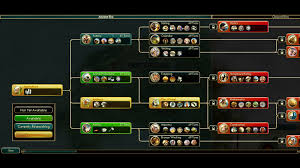
\includegraphics{civ5_tech_tree}
	\caption{Výřez stromu technologií ze hry Civilisation~V \citep{site:civ5}}
	\label{fig:civ5techtree}
\end{figure}


Explicitní strom technologií, viditelný na \ref{fig:civ5techtree}, se v~RTS hrách vyskytuje spíše výjimečně. Nejčastěji je odemykání nových typů jednotek a~budov umožněno stavbou určitého typu budovy nebo dosažení určitého stupně vylepšení již existující budovy. Jako příklad můžeme vzít Warcraft~3 \citep{site:warcraft3}, kde závislosti budov na stupních vylepšení a~existenci jiných budov tvoří strom technologií. Graf tvořený těmito závislostmi můžeme vidět na obrázku \ref{fig:warcrafttechtree}. Zde vidíme stupně vylepšení budov, reprezentované šedými šipkami, a~závislosti budov na ostatních budovách a~stupních jejich vylepšení. Aby byl hráč schopen postavit budovu, musí vlastnit všechny budovy na kterých je tato budova závislá v~požadovaném nebo lepším stupni vylepšení. Ve hře je tento graf reprezentován požadavky zobrazenými při najetí myší na ikonu zamčené budovy.

\begin{figure}[h]	
	\centering
	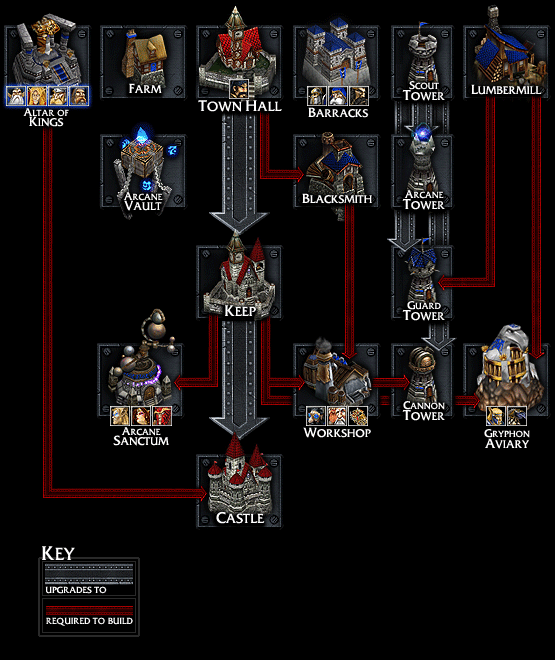
\includegraphics{warcraft_tech_tree}
	\caption{Budovy a~závislosti mezi nimi tvořící obdobu stromu technologií ve hře Warcraft 3}
	\label{fig:warcrafttechtree}
\end{figure}

Jak bylo řečeno v~sekci o~budovách \ref{sec:budovy}, naše platforma bude umožňovat tvůrci postupné odemykání budov a~jednotek, což umožní tvůrci her implementovat výzkum nových technologií. Pro technologie měnící vlastnosti typů jednotek bude pouze na tvůrci, aby změnil logiku hry a~chování umělé inteligence v~závislosti na vyzkoumaných technologiích.

\subsubsection{Shrnutí požadavků}
\label{sec:requirements}

\noindent{Naše platforma bude podporovat tyto vlastnosti:}
\begin{itemize}
	\item[\textbf{T1:}] postupné odemykání budov a~jednotek,
	\item[\textbf{T2:}] změny chování a~vlastností jednotek v~průběhu hry.
\end{itemize}

\section{Uživatelé}
V předešlé sekci jsme popsali druh her, který bude naše platforma podporovat. V~této sekci popíšeme požadavky na chování platformy z~pohledu všech druhů našich uživatelů.

\subsection{Tvůrci her}
Prvním druhem uživatele budou tvůrci her, používající naši platformu pro zjednodušení své práce a~vyřešení problémů opakujících se ve většině RTS her. Tvůrce samozřejmě nemusí být pouze jeden člověk, vzhledem ke složitosti RTS her existuje při jejich tvorbě mnoho rolí, které požadují velmi různorodé schopnosti a~mohou být plněny více lidmi. Příkladem rolí může být 3D umělec tvořící modely a~animace, producent hudby, tvůrce umělé inteligence, programátor herní logiky a~nakonec člověk, který toto vše integruje dohromady.

\subsubsection{Programátor}
Naším hlavním cílem je umožnit tvůrcům umělé inteligence a~programátorům herní logiky použít všechny jazyky .NET Frameworku, především C\#, pro jejich práci. Z~programátorského pohledu bude naše platforma sloužit jako knihovna poskytující tyto funkce:

\begin{enumerate}
	\item udržování aktuálního stavu hry a zjišťování tohoto stavu;
	\item vytváření nových jednotek, budov a~projektilů;
	\item registrování metod, které budou zavolány při určitých událostech v~průběhu hry;
	\item úpravu terénu jak v editoru, tak při běhu hry;
	\item vykreslování terénu, jednotek, budov, projektilů a~grafického rozhraní;
	\item ukládání a~načítání stavu hry;
	\item implementaci řešení pro základní problémy jako pohyb po terénu, let projektilů a~výpočet úhlu střelby projektilů;
	\item ovládání kamery.
\end{enumerate}

Protože implementace vykreslování a~grafického rozhraní by byla nad rámec jedné bakalářské práce, využije naše platforma pro tyto účely existující herní engine UrhoSharp. Pro programátory následně  poskytneme přístup k~relevantním částem UrhoSharp enginu.

Platforma bude poskytovat ovládání kamery v~několika módech. Tato funkcionalita bude potřebná již pro implementaci editoru, poskytneme ji tedy i~tvůrcům her. Prvním módem bude klasická RTS top-down kamera, jakou můžete vidět na ukázce ze hry Company of Heroes \ref{fig:cohcamrts}. Kamera je umístěna v~dostatečné vzdálenosti pro zobrazení celých skupin jednotek, skloněna zhruba 45 stupňů od horizontální polohy.  Ve hře Company of Heroes je ovšem oproti jiným starším RTS hrám jako Warcraft 3 nebo Age of Empires 3 s~kamerou možné rotovat a~přibližovat, což nám přijde jako velice atraktivní. Příklad tohoto pohybu kamery můžete vidět na obrázku \ref{fig:cohcamcin}, kde můžeme vidět pohled z~Německé strany na vylodění na pláži Omaha. Toto bychom rádi podporovali i~v~naší platformě. Druhým módem kamery bude tzv. \uv{free-float} , kdy kamera volně \uv{létá}  nad terénem. Třetím módem bude sledování jednotky, kdy se kamera bude chovat jako v~prvním módu, její pohyb bude ale řízen pohybem jednotky.

\begin{figure}[h]	
	\centering
	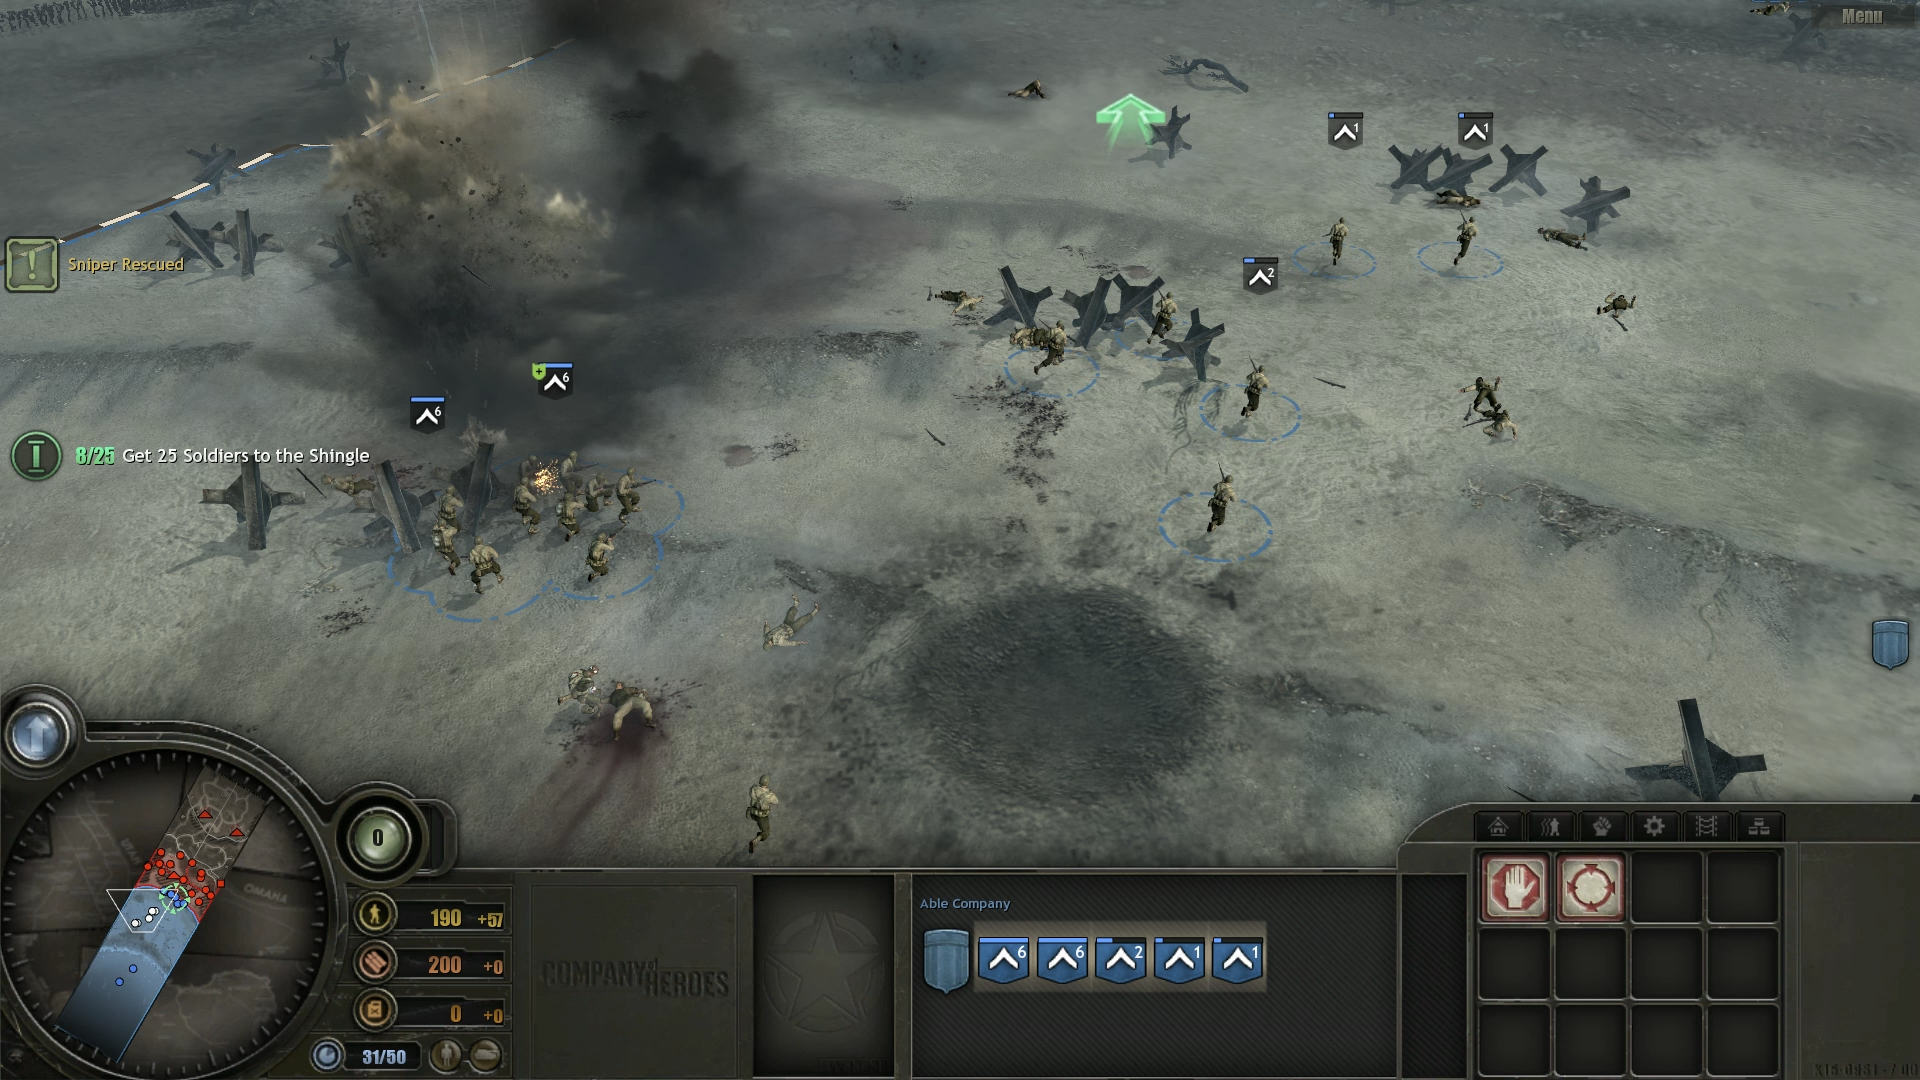
\includegraphics[scale=0.2]{cohcamrts}
	\caption{Klasický RTS pohled kamery ve hře Company of Heroes}
	\label{fig:cohcamrts}
\end{figure}

\begin{figure}[h]	
	\centering
	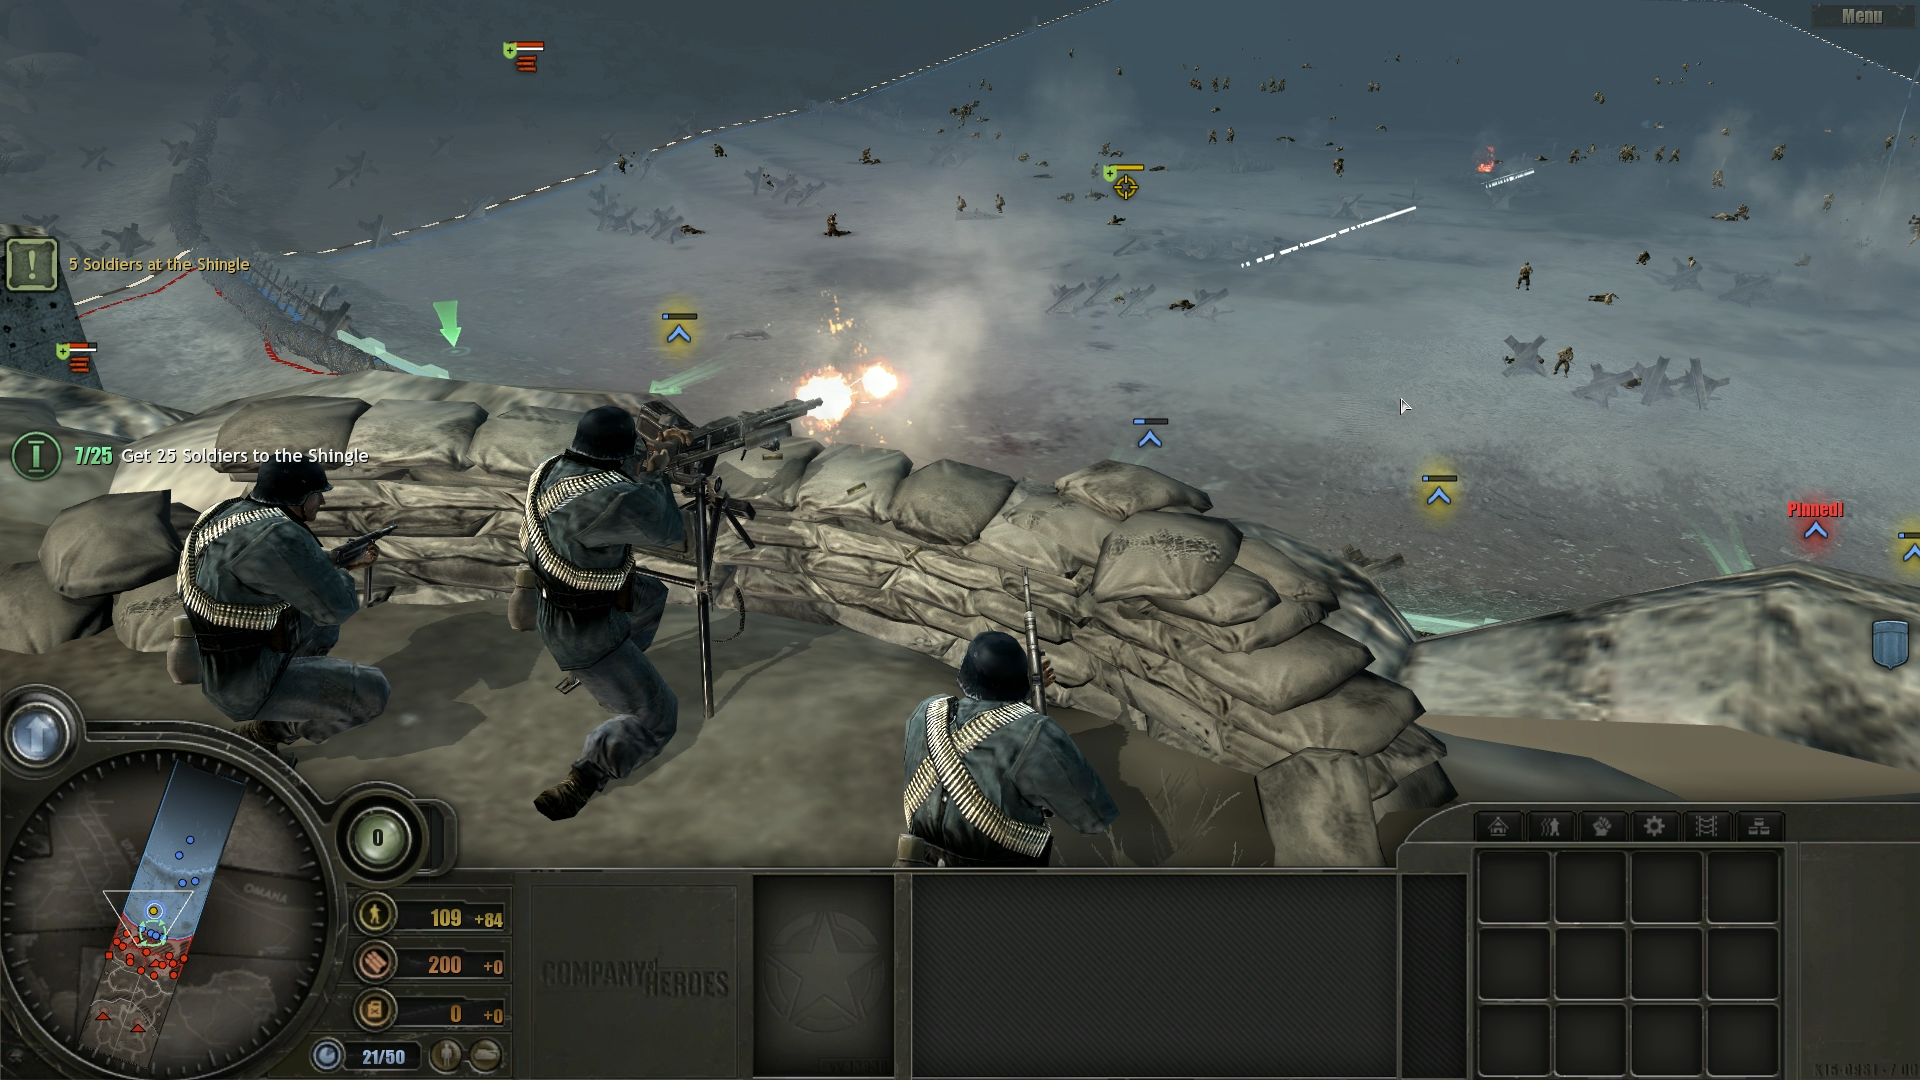
\includegraphics[scale=0.2]{cohcamcin}
	\caption{Co lze vidět s~pouhým přibližováním a~otáčením kamery hře Company of Heroes}
	\label{fig:cohcamcin}
\end{figure}

\subsubsection{Moddeři}

Pro integraci vytvořených jednotek, budov, dlaždic a~jejich modelů, textur a~logiky umožní naše platforma vytvořit \emph{balíček}, obsahující vše vytvořené programátory a~umělci.  Tento balíček poté platforma umožní přidat a~načíst v~libovolné instalaci platformy.

Platforma bude také sloužit jako editor úrovní, které budou využívat logiku, jednotky, budovy a~typy terénu dodané pomocí balíčků. Vytvořené úrovně bude následně možné uložit zpět do balíčku a~distribuovat spolu s~balíčkem do dalších instancí naší platformy.

Pro editaci mapy poskytne platforma několik základních nástrojů a~umožní tvůrcům modifikovat nástroje či přidávat své vlastní. Základní nástroje by měli umožnit editaci terénu mapy (změnu typu terénu na všechny tvůrci definované typy a~editaci výšky dlaždic) a~přidávání všech druhů jednotek a~budov do mapy.

Formát ukládání úrovní bude definován otevřeně pomocí prostředků nezávislých na programovacím jazyce, čímž chceme umožnit tvorbu separátních editorů map produkujících úrovně v~námi používaném formátu.

\subsection{Hráči her}
Z pohledu hráče se bude platforma chovat jako instalovatelná aplikace, která hráči umožní za běhu přidávat balíčky a~následně využít jejich obsah.

Při běhu platforma umožní plný přístup k~nastavení UrhoSharp enginu, tedy k~nastavení rozlišení, Vsync, triple buffer a~dalších. Dále umožní správu balíčků, tedy přidávání, odebírání a~spouštění. Při spuštění balíčku umožní platforma hráči výběr z~existujících map, jak pro hraní, tak pro editaci. Dále platforma umožní vytvoření a~editaci úplně nové mapy.

Při tvorbě nové mapy či editaci existující mapy mít bude hráč přístup ke všem jednotkám, budovám a~typům terénu, ke kterým mu dají editační nástroje specifikované tvůrcem balíčku přístup. Následně bude hráči umožněno mapu uložit, a~to přepsáním zdrojové mapy, kterou hráč načetl k~editaci, nebo vytvořením nové mapy pod novým jménem.

\section{Ukázková hra}
\label{sec:showcasedef}

Pro ukázku bude vytvořen balíček s~jednoduchou hrou demonstrující možnosti naší platformy. Ukázková hra bude zároveň sloužit jako referenční příklad použití naší platformy.

\noindent{\textbf{Ukázková hra bude obsahovat několik jednotek, demonstrujících tyto vlastnosti:}}
\begin{enumerate}
	\item jednoduchou a~složitější umělou inteligenci;
	\item plně automatické jednotky, neovladatelné hráčem;
	\item jednotky útočící na dálku;
	\item jednotky útočící na blízko;
	\item aktivní získávání surovin;
	\item pohyb po terénu;
	\item pohyb nad terénem (létání);
	\item rozdílnou rychlost pohybu různých jednotek;
	\item rozdílnou přístupnost částí mapy pro různé jednotky;
	\item pohyb po budovách.
\end{enumerate}

\noindent{\textbf{Demonstrovanými vlastnostmi budov budou:}}
\begin{enumerate}
	\item restrikce na umístění stavby,
	\item neprostupnost budov pro některé jednotky;
	\item produkce surovin budovami;
	\item přidání plochy nebo části plochy budovy jako přístupný terén pro určité typy jednotek.
\end{enumerate}

\noindent{\textbf{Jako obecné vlastnosti bude ukázková hra demonstrovat:}}
\begin{enumerate}
	\item RTS mód kamery,
	\item volný pohyb kamery,
	\item sledování jednotky kamerou,
	\item tvůrcem definované prvky v~uživatelském rozhraní,
	\item minimapu.
\end{enumerate}

\noindent{\textbf{Balíček obsahující ukázkovou hru bude demonstrovat tyto vlastnosti:}}
\begin{enumerate}
	\item tvorbu vlastních úrovní za použití jednotek, budov a~typů terénu obsažených v~balíčku;
	\item ukládání a~načítání hry.
\end{enumerate}

\section{Cíle práce}
\label{sec:cileprace}
Cílem této práce je vytvořit platformu pro vývoj 3D RTS her pro jednoho hráče za použití herního enginu UrhoSharp, umožňující vývojářům vytvářet hry jako separátně 
distribuované balíčky, které bude poté koncový uživatel schopen přidat do naší platformy nainstalované na uživatelově počítači a~použít je pro hraní dodaných úrovní či tvorbu svých vlastních.

Při tvorbě hry bude umožněno tvůrci použít jazyky frameworku .NET  pro vytvoření Umělé inteligence jednotek, budov a~nepřátelských hráčů, pro vytvoření další logiky hry a~pro přidání nástrojů do editoru map. 

\noindent{\textbf{Požadované vlastnosti platformy:}}
\begin{enumerate}
	\item podporované vlastnosti jednotek:
		\begin{enumerate}
			\item pohyb jednotek (J1, J2)
			\item ovládání jednotek (J3, J4)
			\item umělá inteligence, definice chování (J5)
			\item produkce jednotek (J6)
			\item přidávání jednotek jako součást úrovně (J7, J8)
			\item podpora systému hit-pointů (J9)
			\item útoky na blízko i~na dálku (J10, J11)
		\end{enumerate}
	\item podporované vlastnosti budov:
		\begin{enumerate}
			\item stavba budov v~herním světě (B1, B9, B10)
			\item podpora obraných budov (B2, B4)
			\item rozšiřitelnost dostupného terénu o~plochu budov (B3)
			\item přidávání budov jako součásti mapy (B5, B6)
			\item zničitelnost budov (B7, B8)
			\item produkce jednotek, surovin, stavba budov pomocí budovy (B11)
		\end{enumerate}
	\item podporované vlastnosti surovin:
		\begin{enumerate}
			\item přidávání a~odebírání libovolného množství surovin (nejen celočíselných) (S1, S2)
		\end{enumerate}
	\item podporované vlastnosti výzkumu technologií:
		\begin{enumerate}
			\item postupné odemykání dostupných jednotek a~budov, umožnit změny chování jednotek za běhu (T1, T2)
		\end{enumerate}
	\item podporované vlastnosti mapy
		\begin{enumerate}
			\item rozdělení mapy na dlaždice (M1)
			\item tvorbu terénu pomocí různých výšek dlaždic. (M2)
			\item různé typy dlaždic. (M3)
			\item rozhraní pro získání aktuálního stavu mapy (jednotek a budov na dlaždici, typu dlaždice ...) (M4, M5)
		\end{enumerate}
	\item vlastnosti pro tvůrce balíčků:
		\begin{enumerate}
			\item platforma musí umožňovat přidávání balíčků za běhu, obsahujících nové typy jednotek, budov,  dlaždic, projektilů a~hráčů spolu s~jejich modely, texturami a~AI
			\item platforma musí umožňovat použití přidaných balíčků pro tvorbu map a~uložení vytvořených map do balíčku použitého pro jejich tvorbu
			\item editor map musí být rozšiřitelný o~nástroje z~balíčku
			\item herní grafické rozhraní musí umožňovat tvůrci přidávat vlastní okna, tlačítka a~další prvky
		\end{enumerate}
	\item vlastnosti pro koncového hráče:
		\begin{enumerate}
			\item uživatelské rozhraní pro stolní počítače, umožňující vybírání balíčků, map a~oponentů, dále načítání a~ukládání her, a~nastavování zobrazení hry
			\item herní uživatelské rozhraní musí obsahovat minimapu, poskytující hráči přehled o~větší části mapy než kterou vidí vlastní kamerou
			\item ovládání kamery umožňující klasický top-down pohled, volné poletování kamery po mapě a~následování jednotky
			\item ukládání a~načítání hry
		\end{enumerate}
\end{enumerate}
